\documentclass{article}
\usepackage[T1]{fontenc}
\usepackage[latin2]{inputenc}
\usepackage[english]{babel}
\usepackage{tikz}
\usetikzlibrary{calc,through,backgrounds,positioning,fit}
\usetikzlibrary{shapes,arrows,shadows}
 
\begin{document}
 
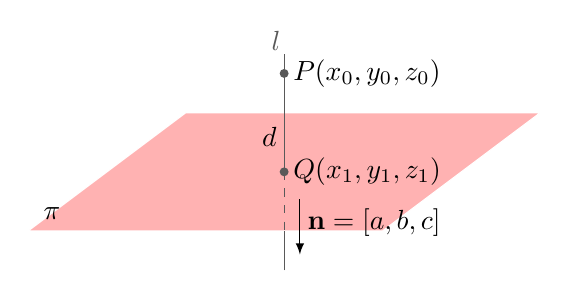
\begin{tikzpicture}[scale=1,inner sep=0.4mm]
\filldraw [fill=red!30!white, draw = white] (0,0,0) -- (4.5,0,0) -- (6.5,1.5,0)  -- (2,1.5,0) -- cycle;
\draw [black!65!white] (3.25,0.75) -- (3.25,2.25) node [above left] {$l$};
\draw [dashed,black!65!white] (3.25,0.75) -- (3.25,0) ;
\draw [black!65!white] (3.25,-0.5) -- (3.25,0);
\draw [- latex,black,thin] (3.45,0.4) -- (3.45,-0.3);
\draw (3.5,0.1) node[right] {$\mathbf n = [a,b,c]$};
\draw (3.2,1.2) node[left] {$d$};
\draw (0.15,0.1) node[above right] {$\pi$};
\node at (3.25,2) [circle,fill=black!65!white] {};
\node at (3.25,2) [right=2pt] {$P(x_0,y_0,z_0)$};
\node at (3.25,0.75) [circle,fill=black!65!white] {};
\node at (3.25,0.75) [right=2pt] {$Q(x_1,y_1,z_1)$};

\end{tikzpicture}
 
\end{document}